\documentclass[12pt, a4paper]{article}

% ── Encoding & fonts ──────────────────────────────────────────────────────────
\usepackage[T1]{fontenc}
\usepackage[utf8]{inputenc}
\usepackage{lmodern}

% ── Page layout ───────────────────────────────────────────────────────────────
\usepackage[
    top=2.5cm, bottom=2.5cm,
    left=3cm,  right=2.5cm
]{geometry}
\usepackage{setspace}
\onehalfspacing

% ── Maths ─────────────────────────────────────────────────────────────────────
\usepackage{amsmath}
\usepackage{amssymb}

% ── Figures & tables ──────────────────────────────────────────────────────────
\usepackage{graphicx}
\usepackage{booktabs}
\usepackage{caption}
\usepackage{float}
\usepackage{multirow}

% ── Hyperlinks & cross-references ─────────────────────────────────────────────
\usepackage[
    colorlinks = true,
    linkcolor  = black,
    citecolor  = black,
    urlcolor   = blue
]{hyperref}

% ── References ────────────────────────────────────────────────────────────────
\usepackage[
    backend  = biber,
    style    = apa,
    sorting  = nyt
]{biblatex}
\addbibresource{references.bib}

% ── Misc ──────────────────────────────────────────────────────────────────────
\usepackage{microtype}
\usepackage{parskip}

% Convenience macro for the information set / conditional-mean notation
\newcommand{\E}{\mathbb{E}}

% ─────────────────────────────────────────────────────────────────────────────
\begin{document}

% ─────────────────────────────────────────────────────────────────────────────
%  Title page
% ─────────────────────────────────────────────────────────────────────────────
\begin{titlepage}
    \centering
    \vspace*{1.2cm}

    {\large IE University} \\[0.25cm]
    {\large Master in Business Analytics \& Data Science} \\[2.6cm]

    {\large\scshape Master's Thesis} \\[1.0cm]

    \rule{\textwidth}{0.4pt} \\[0.65cm]
    {\LARGE\bfseries Mean, Variance, and Market Efficiency \\[0.35cm]
    in the Silver Market\par}
    \vspace{0.65cm}
    {\large\itshape Forecasting Weekly Returns and Realised Volatility with
    Classical, \\[0.15cm] Machine-Learning, and Deep-Learning Models\par}
    \vspace{0.55cm}
    \rule{\textwidth}{0.4pt} \\[2.4cm]

    {\large Asier Ugarteche Perez} \\[1.6cm]

    {\normalsize Supervisor: Prof.\ Dae-Jin Lee} \\[0.4cm]

    \vfill
    {\normalsize Academic Year 2025/2026}
\end{titlepage}
\thispagestyle{empty}

% ── Abstract ──────────────────────────────────────────────────────────────────
\begin{abstract}
\noindent
% DRAFT abstract — qualitative, to be finalised once all results tables are frozen.
This thesis asks how much of silver's short-term price behaviour can be forecast, and
frames the question through the efficient-market hypothesis (EMH). Silver is modelled at
the weekly (Friday-to-Friday) horizon over 2015--2026, and the analysis is factorised
into the two moments: the conditional \emph{mean} of returns and the conditional
\emph{variance}---efficiency constrains the former but not the latter. For the mean, a
deliberate ladder of models of increasing flexibility---ARIMA/ARIMAX, VAR,
mixed-data-sampling (MIDAS) regressions, random forests, gradient boosting, and an
LSTM---is tested against a common random-walk-with-drift benchmark, expanding the
information set from silver's own past (weak-form EMH) to a broad set of public
information (semi-strong-form EMH): cross-asset returns, silver futures positioning,
macroeconomic releases, technical indicators, and sentiment from Reddit and financial
news. For the variance, weekly realised volatility is modelled with GARCH and the
heterogeneous autoregressive (HAR) model, and the question of interest is whether
sentiment improves the forecast. The central finding is a single coherent statement: no
model beats the drift benchmark for the conditional mean by a significant
margin---weak- and semi-strong-form efficiency hold for weekly silver returns---yet the
conditional variance is strongly and significantly forecastable, with sentiment adding a
small but robust increment. Predictable volatility alongside an unpredictable mean is
exactly what the EMH permits, so the two results are complementary rather than
contradictory.
\end{abstract}

\newpage
\thispagestyle{empty}

% ── Table of contents ─────────────────────────────────────────────────────────
\tableofcontents
\newpage

% ═════════════════════════════════════════════════════════════════════════════
\section{Introduction}
\label{sec:intro}
% ═════════════════════════════════════════════════════════════════════════════

Silver lives a double life. It is an industrial input---roughly half of annual demand
goes into photovoltaics, electronics, brazing alloys, and medical uses, tying its price
to the global manufacturing cycle---and, at the same time, a monetary metal held as a
store of value, an inflation hedge, and a more volatile cousin of gold. On top of both
sits a retail following that can sometimes turn silver into a meme trade: in late January
2021, Reddit's r/WallStreetSilver drove spot from roughly \$25 to \$30 an ounce within
days before it faded. This blend of industrial demand, monetary hedging, and episodic
retail attention makes silver an unusually rich laboratory for the oldest question in
empirical finance: how much of a price can be forecast?

That question has a canonical answer, and it is mostly negative. The efficient-market
hypothesis \parencite{fama1970,fama1991} holds that prices already embed available
information, so successive price changes are approximately unpredictable. It is conventionally stated in three nested forms, graded by the
information set a forecaster is allowed to use:

\begin{itemize}
    \item \textbf{Weak form} --- past prices and returns carry no exploitable signal.
    \item \textbf{Semi-strong form} --- no \emph{public} information does either: not
    prices, fundamentals, news, or macroeconomic data.
    \item \textbf{Strong form} --- not even \emph{private}, inside information does.
\end{itemize}

\noindent Each form nests the one before it, so the claims grow progressively stronger.
For a liquid, globally traded metal, weak- and semi-strong-form efficiency are the
natural hypotheses to take to the data, and they are the two this thesis tests.

Empirically, silver's \emph{price} behaves like a random walk with drift: it is
non-stationary, and shocks accumulate rather than mean-revert
(Figure~\ref{fig:silver-price}). Returns, however, are stationary---they fluctuate around
a stable long-run mean rather than wandering without bound. The object worth modelling is
therefore not the price level but its increment, the weekly log-return
\(r_t = \log P_t - \log P_{t-1}\); stationarity is what makes the forecasting problem
well-posed, giving a fixed quantity to predict and a natural yardstick---that same
prevailing average---to judge any forecast against.

% TEMP: colour-marked — delete this {\color{red} ... } wrapper (or the whole paragraph)
{\color{red}
The weekly (Friday-to-Friday) horizon is a deliberate choice of frequency, made where the
information aligns. Futures-market positioning is reported weekly and macroeconomic
releases monthly, while daily sentiment is too sparse and noisy to inform a forecast and
daily returns are dominated by microstructure noise; a weekly horizon is coarse enough to
average out that noise yet fine enough to leave roughly six hundred observations over
2015--2026---enough to train and properly out-of-sample-test the machine-learning models.
Weekly realised volatility, the target of the second-moment analysis, is in turn
aggregated from daily returns.
}

\begin{figure}[htbp]
    \centering
    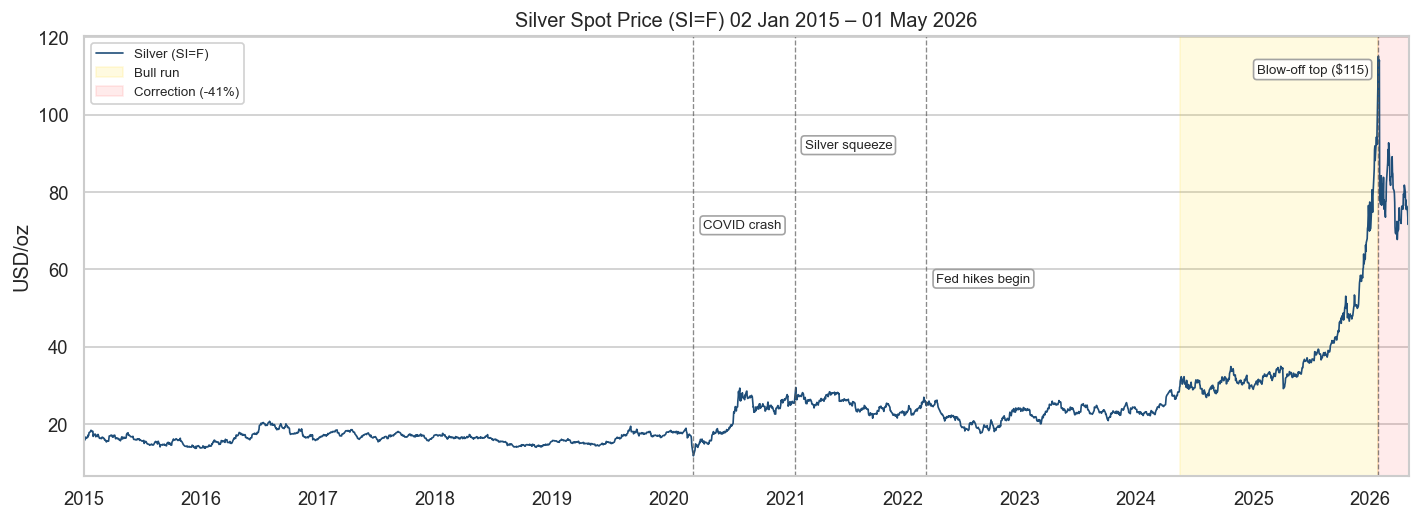
\includegraphics[width=\textwidth]{images/output.png}
    \caption{Silver front-month futures (SI=F), daily, January 2015--May 2026. The
    annotated episodes punctuate the sample: the COVID-19 crash (March 2020), the
    r/WallStreetSilver squeeze (January 2021), the start of the Federal Reserve's hiking
    cycle (March 2022), and the 2024--2026 bull run that carried spot to an all-time high
    near \$115/oz before a sharp ($-41\%$) correction. The level is non-stationary and
    shocks accumulate; the thesis models its stationary weekly log-return rather than the
    level itself.}
    \label{fig:silver-price}
\end{figure} The efficiency question then becomes whether \(r_t\)
can be forecast---and silver's own past offers little to go on. Weekly
returns carry almost no linear autocorrelation, so a linear own-history model such as
ARIMA has little to grip; a formal model search duly collapses it to a constant mean. Yet
the returns are not independent noise either, because their \emph{magnitude} is
persistent---volatile weeks cluster together---so structure remains, only in the variance
rather than the mean. The thesis follows this thread: it asks first whether silver's own
history forecasts the return, then whether the broad public-information set a real
forecaster would possess does---cross-asset returns (gold, the US dollar, copper,
equities, oil, and the VIX), futures-market positioning, macroeconomic releases,
technical indicators, and retail and news sentiment---and, separately, whether the
predictable variance can be modelled.

\textbf{Research questions.} The thesis is built around four questions:
\begin{itemize}
    \item \textbf{Q1 (weak form).} Are weekly silver returns forecastable from their
    own past?
    \item \textbf{Q2 (semi-strong form).} Does expanding the information set to public
    covariates help---and does it matter whether the relationship is assumed linear or
    allowed to be nonlinear?
    \item \textbf{Q3 (the second moment).} Is weekly realised volatility forecastable,
    and if so by how much?
    \item \textbf{Q4 (sentiment).} Does retail and news sentiment add incremental
    predictive content to either the conditional mean or the conditional variance?
\end{itemize}

\textbf{Approach.} To answer these questions, the analysis works at the weekly
(Friday-to-Friday) horizon and estimates a deliberate ladder of models of increasing
flexibility against a common benchmark and a unified evaluation protocol. The benchmark
throughout is the prevailing-mean ``drift'' forecast---the random-walk-with-drift,
equivalent to ARIMA(0,0,0)---which is the correct null for a return target
\parencite{welch2008,campbell2008}. For the conditional mean, the ladder runs from
classical time-series models (ARIMA/ARIMAX, VAR, and MIDAS regressions) through tree
ensembles (random forests and gradient boosting) to a recurrent neural network (LSTM);
for the conditional variance it runs GARCH and the heterogeneous autoregressive (HAR)
model of \textcite{corsi2009} alongside the same tree ensembles. Forecasts are compared
on out-of-sample \(R^2\) relative to the drift \parencite{campbell2008}, the
Diebold--Mariano test of equal predictive accuracy \parencite{diebold1995}, and the
Pesaran--Timmermann test of directional accuracy \parencite{pesaran1992}, all on a
held-out 2023--2026 test window.

% TEMP: colour-marked — delete this {\color{red} ... } wrapper (or the whole paragraph)
{\color{red}
\textbf{Structure.} The remainder of the thesis is organised as follows.
Section~\ref{sec:framework} sets out the conceptual framework---the random-walk view of
prices, the martingale-difference characterisation of the conditional mean, the
expanding information set, and the linear-versus-nonlinear alternatives that motivate the
model ladder. Section~\ref{sec:lit} reviews the relevant literature on commodity-return
predictability, mixed-frequency modelling, realised-volatility forecasting, and financial
sentiment. Section~\ref{sec:data} describes the data and feature construction.
Section~\ref{sec:method} presents the models and the unified evaluation protocol.
Section~\ref{sec:mean} reports the conditional-mean (returns) results, and
Section~\ref{sec:var} the conditional-variance (volatility) results.
Section~\ref{sec:discussion} discusses the findings against the efficiency framing, and
Section~\ref{sec:conclusion} concludes with limitations and directions for future work.
}

% ═════════════════════════════════════════════════════════════════════════════
\section{Conceptual Framework}
\label{sec:framework}
% ═════════════════════════════════════════════════════════════════════════════

% PLACEMENT NOTE (for the author): this section is the home of the random-walk /
% martingale-difference / information-set notation. The intro states the efficiency
% question in plain English; this section gives it the precise form that motivates the
% model ladder; the Conclusion (sec:conclusion) revisits the one-paragraph synthesis.
% Drafted concisely below; expand per notebooks/weekly/formulas.md as needed.

This section fixes the notation used throughout and states, precisely, the nulls that
each model class is built to test. The aim is to keep the language exact without
overclaiming: the empirical results are framed as tests of the conditional mean and the
conditional variance of weekly silver returns, not as claims about the full return
distribution.

\subsection{Prices, returns, and the random walk}
\label{sec:framework-rw}

Let \(P_t\) be the silver price and \(p_t = \log P_t\) the log price. The weekly
log-return is the increment in the log price,
\begin{equation}
    r_{t+1} = p_{t+1} - p_t, \qquad\text{equivalently}\qquad p_{t+1} = p_t + r_{t+1},
\end{equation}
so the price level and the return are two views of the same process: the level
accumulates shocks, while returns \emph{are} the shocks. A random walk with drift writes
the level as \(p_{t+1} = p_t + \mu + \varepsilon_{t+1}\) with
\(\E[\varepsilon_{t+1}] = 0\). Silver log prices are best described as
\emph{random-walk-like}---non-stationary, with shocks that accumulate---which is the
reason the modelling target throughout is the stationary increment \(r_t\) rather than
the level. The safer wording avoids the \emph{strict} random walk: the innovations are
not independent and identically distributed, because their variance clusters
(Section~\ref{sec:framework-var}).

\subsection{The conditional mean and the information set}
\label{sec:framework-mds}

Let \(F_t\) denote the information available at time \(t\). For the weak-form test, this
is silver's own past, \(F_t = \{r_t, r_{t-1}, r_{t-2}, \dots\}\). Returns satisfy the
\emph{martingale difference} property with respect to \(F_t\) if their conditional mean is
constant,
\begin{equation}
    \E[r_{t+1} \mid F_t] = \mu,
    \label{eq:weak-null}
\end{equation}
or, equivalently, the demeaned return \(r_{t+1} - \mu\) is a \emph{martingale difference
sequence} (MDS),
\begin{equation}
    \E[r_{t+1} - \mu \mid F_t] = 0.
    \label{eq:weak-null-mds}
\end{equation}
Past returns do not move the expected next-week return away from its long-run average.
This is a statement about the first moment \emph{only}; it does not assert that returns
are i.i.d. The semi-strong test expands the information set to public covariates,
\begin{equation}
    G_t = \{F_t,\ \text{gold},\ \text{USD},\ \text{copper},\ \text{VIX},\ \text{oil},\
    \text{COT},\ \text{macro},\ \text{technicals},\ \text{sentiment}\},
\end{equation}
and asks whether the martingale-difference property survives the larger conditioning set,
\begin{equation}
    \E[r_{t+1} \mid G_t] = \mu.
    \label{eq:ss-null}
\end{equation}
ARIMA tests whether silver returns are a martingale difference with respect to their own
past, Equation~\eqref{eq:weak-null}; ARIMAX and the other models test whether
that property survives once the information set is expanded to public covariates,
Equation~\eqref{eq:ss-null}. Operationally, these nulls are tested as ``does the model
beat the prevailing-mean (drift) benchmark out of sample?''---a forecast that beats the
drift would contradict the corresponding null.

\subsection{Linear and nonlinear alternatives}
\label{sec:framework-nonlin}

The alternative to Equation~\eqref{eq:ss-null} can be specified narrowly or broadly. A
linear model entertains an additive alternative,
\begin{equation}
    \E[r_{t+1} \mid G_t] = \mu + \beta' G_t,
\end{equation}
so ARIMAX, VAR, and MIDAS ask whether public covariates enter the conditional mean
linearly and additively. Nonlinear models entertain the broader alternative
\begin{equation}
    \E[r_{t+1} \mid G_t] = f(G_t),
\end{equation}
where \(f\) may encode thresholds, interactions, regime dependence, and sequence
effects. The motivation is concrete: a signal may be invisible to any single covariate
yet present in a combination. Each condition alone may carry little signal,
\(\E[r_{t+1}\mid \text{high sentiment}] \approx \mu\) and
\(\E[r_{t+1}\mid \text{stretched COT}] \approx \mu\), while the joint condition does not,
\begin{equation}
    \E\!\left[r_{t+1}\mid \text{high sentiment},\ \text{stretched COT},\
    \text{rising VIX},\ \text{falling USD}\right] \neq \mu .
\end{equation}
Random forests, gradient boosting, and the LSTM search this larger space.
The logic of the ladder is therefore cumulative: if even flexible nonlinear models fail
to beat the drift benchmark out of sample, the martingale-difference interpretation is
\emph{strengthened} rather than merely assumed from linear tests. A complementary
own-history check, the generalised spectral test \parencite{hong2003}, probes for
nonlinear departures from Equation~\eqref{eq:weak-null} that linear autocorrelation
diagnostics cannot see.

\subsection{The conditional variance}
\label{sec:framework-var}

Efficiency constrains Equation~\eqref{eq:ss-null}; it places no restriction on the
conditional variance \(\operatorname{Var}(r_{t+1}\mid F_t)\). The two can diverge: the
mean may be (approximately) constant while the variance moves through time, which is
exactly what volatility clustering means---a large move today says little about the sign
or size of next week's return but does signal that next week is likely to be more
volatile. Strict white noise would require independence in \(r_t\), \(r_t^2\), and
\(|r_t|\) alike; the MDS property in Equation~\eqref{eq:weak-null} restricts only the
first of these. Weekly silver returns are close to white noise in the mean but not
strict white noise, because squared returns are strongly autocorrelated. The predictable
structure is therefore concentrated in the second moment, which is what the volatility
chapter (Section~\ref{sec:var}) targets directly via realised volatility.
Figure~\ref{fig:returns-acf} shows both moments at once for the weekly silver return.

\begin{figure}[htbp]
    \centering
    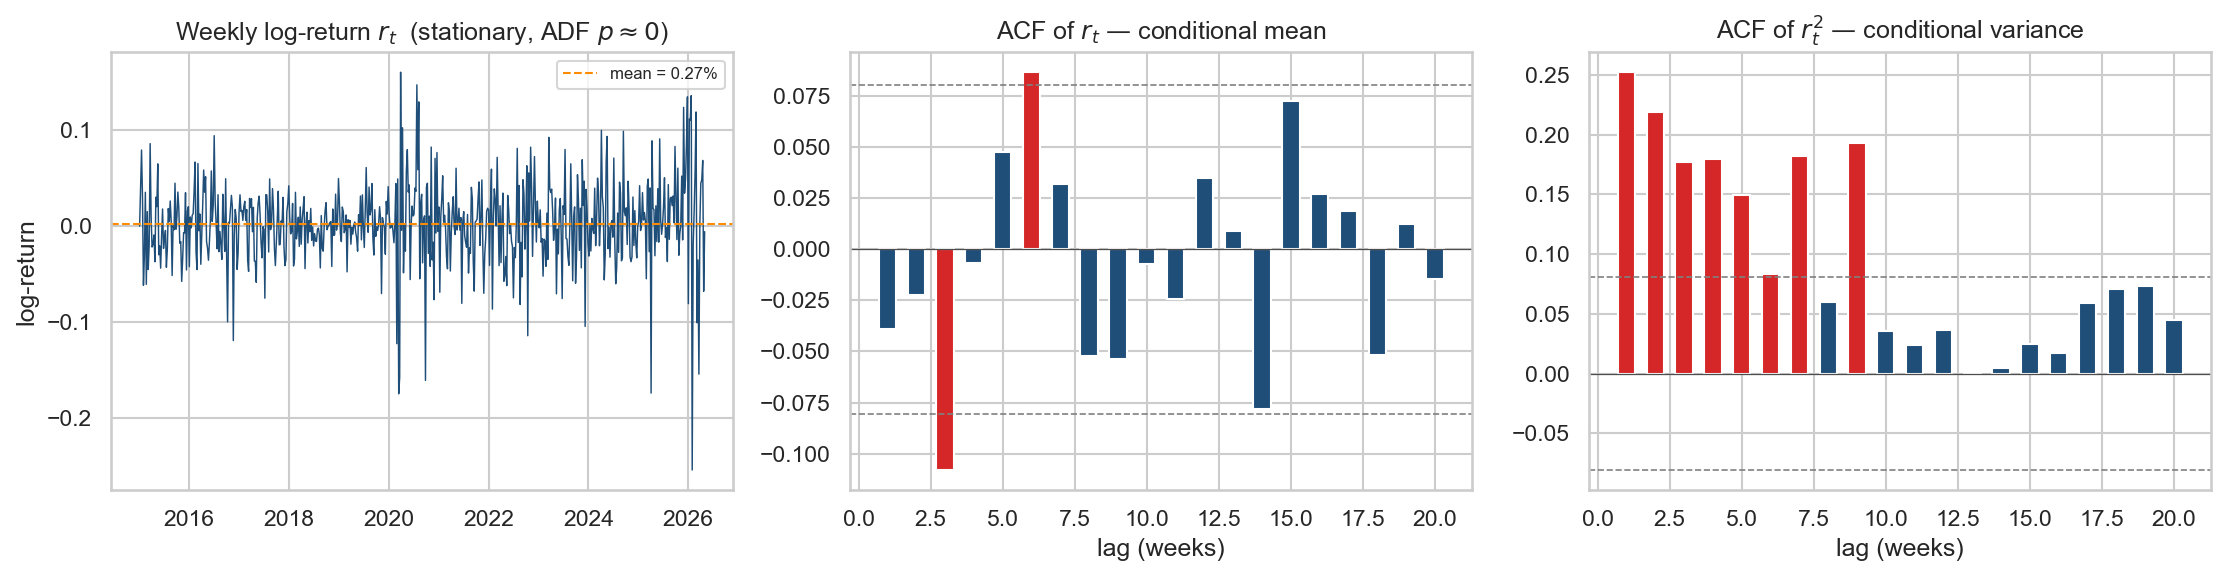
\includegraphics[width=\textwidth]{images/returns_acf.png}
    \caption{The two moments of the weekly silver log-return, 2015--2026. \emph{Left:}
    the return series---stationary, fluctuating around a small positive drift
    (mean \(\approx 0.0027\)/week). \emph{Centre:} the sample autocorrelation of returns
    lies almost entirely within the 95\% white-noise band (dashed), with only isolated
    lags breaching it---consistent with the martingale-difference null of
    Equation~\eqref{eq:weak-null}, so a linear own-history model has little to exploit.
    \emph{Right:} the autocorrelation of \emph{squared} returns is large and positive
    across the first several lags---the volatility clustering of
    Section~\ref{sec:framework-var}. The mean is close to unpredictable; the variance is
    not.}
    \label{fig:returns-acf}
\end{figure}

\subsection{Direction versus magnitude}
\label{sec:framework-direction}

A final distinction governs how forecasts are scored. Directional accuracy asks whether
\(\operatorname{sign}(\hat r_{t+1}) = \operatorname{sign}(r_{t+1})\) more often than
chance, which is \emph{not} the same as beating the drift benchmark under squared-error
loss: a model can call the sign correctly yet fail to improve out-of-sample \(R^2\).
Because efficiency is a conditional-mean claim, the magnitude axis (RMSE, out-of-sample
\(R^2\), and Diebold--Mariano against the drift) is load-bearing, while directional
accuracy---and its significance test, Pesaran--Timmermann \parencite{pesaran1992}---is a
secondary, economically motivated lens. Directional gains are interesting but do not by
themselves reject the martingale-difference null.

% ═════════════════════════════════════════════════════════════════════════════
\section{Literature Review}
\label{sec:lit}
% ═════════════════════════════════════════════════════════════════════════════

The thesis sits at the intersection of five strands of literature: the long empirical
record on commodity-return predictability and market efficiency, mixed-frequency
regression, machine learning for financial forecasting, realised-volatility modelling,
and text-based sentiment. This section reviews each in turn, with an eye on the specific
design choices they motivate in the chapters that follow.

\subsection{Commodity-return predictability and market efficiency}

The efficiency framing of Section~\ref{sec:framework} descends directly from
\textcite{samuelson1965} and the weak/semi-strong/strong taxonomy of
\textcite{fama1970}, whose later survey \parencite{fama1991} reframed the weak form
more broadly as ``tests for return predictability''---precisely the form the present
exercise takes. For commodities specifically, the canonical stylised facts are
discouraging for forecasters: \textcite{deaton1992} document spot prices that are
extremely volatile, dominated by long quiet spells punctuated by sharp spikes, and
difficult to distinguish from highly persistent, near-unit-root processes---which is why
the stationary increment (the return), not the level, is the only defensible modelling
target. At the same time, commodities do not move in isolation:
\textcite{zhang2010} find cointegration and price discovery between crude oil and gold,
and \textcite{batten2010} show that the macroeconomic determinants of volatility differ
across the precious metals, with silver responding to a different mix of monetary
variables than gold. Together these findings motivate the cross-asset information set
used here---gold, the dollar, copper, equities, the VIX, and oil---while cautioning
against treating silver as a small gold.

Whether any of that public information translates into out-of-sample forecasting power
is the subject of a debate the thesis borrows its evaluation protocol from.
\textcite{welch2008} re-examine the full catalogue of variables claimed to predict the
equity premium and find that essentially none beats the prevailing historical mean once
evaluated out of sample; \textcite{campbell2008} reply that modest gains are possible,
but only with theory-imposed restrictions, and propose the out-of-sample \(R^2\) against
the prevailing-mean forecast as the natural yardstick. That benchmark---the
random-walk-with-drift, estimated as an expanding historical mean---and that metric are
adopted unchanged in Section~\ref{sec:method}. Finally, \textcite{lo2004} offers the
adaptive-markets reading in which efficiency is not a binary property but an
evolutionary, time-varying one, so that pockets of predictability can appear and decay;
this is the natural frame for the episodic, non-replicating directional signals
encountered in Section~\ref{sec:mean}.

\subsection{Mixed-frequency models (MIDAS)}

Forecasting a weekly return with monthly macroeconomic releases and daily market data
poses an alignment problem: aggregating the high-frequency series throws information
away, while including every high-frequency lag as a free regressor invites massive
parameter proliferation. Mixed-data-sampling (MIDAS) regression
\parencite{ghysels2004,ghysels2007} resolves the trade-off by letting the
high-frequency lags enter through a low-dimensional weight polynomial---typically the
Beta or exponential-Almon family---so that a long lag window costs two or three
parameters instead of dozens. \textcite{andreou2013} demonstrate the payoff in the
direction most studied, using daily financial data to forecast quarterly macro
aggregates; the present application inverts that direction, bringing monthly macro
releases and daily cross-asset returns to bear on a weekly financial target. The
\texttt{midasr} package \parencite{ghysels2016r} documents the now-standard estimation
approach---nonlinear least squares over the weight parameters with the linear
coefficients profiled out---which the Python implementation in this thesis follows.

\subsection{Machine learning and deep learning for financial time series}

Tree ensembles and recurrent neural networks instantiate the nonlinear alternative
\(f(G_t)\) of Section~\ref{sec:framework-nonlin}: random forests and gradient boosting
capture thresholds and interactions without specifying them in advance, and the long
short-term memory network \parencite{hochreiter1997} adds explicit sequence memory,
extracting its own representation of the recent past rather than consuming hand-picked
lags. The applied literature is large and, on its face, encouraging---the systematic
review of \textcite{sezer2020} catalogues hundreds of deep-learning forecasting studies
reporting gains over classical models. It is also methodologically uneven: benchmarks
are often weak or absent, evaluation windows short, and statistical significance rarely
assessed, so reported out-performance frequently dissolves against an honest no-change
or prevailing-mean benchmark. The design response in this thesis is to keep the model
ladder flexible but the referee strict: every learner, however expressive, is scored
against the same drift benchmark with the same Diebold--Mariano test, so that
flexibility can only ever strengthen---never substitute for---the efficiency verdict.

\subsection{Realised volatility and the HAR model}

That the conditional variance, unlike the conditional mean, is forecastable has been
textbook knowledge since \textcite{engle1982} introduced ARCH and \textcite{bollerslev1986}
generalised it: volatility clusters, so its own past predicts it. The realised-volatility
literature sharpened the target, replacing latent variance with a model-free estimate
built from higher-frequency squared returns---here, weekly realised volatility from
daily returns. Its workhorse forecaster is the heterogeneous autoregressive (HAR) model
of \textcite{corsi2009}, which regresses next period's realised volatility on its own
past averaged over short, medium, and long horizons; despite being estimable by OLS, the
cascade of horizons approximates the long memory of volatility well enough that HAR
remains the standard benchmark. Evaluation has its own subtlety: realised volatility is
itself a noisy proxy of the latent target, and \textcite{patton2011} shows that only a
restricted family of loss functions---in practice MSE and QLIKE---ranks forecasts
consistently under proxy noise, with QLIKE the more powerful in heavy-tailed samples.
The volatility chapter therefore reports QLIKE-based Diebold--Mariano tests as primary.
None of this strains the efficiency hypothesis, which constrains the mean and not the
variance (Section~\ref{sec:framework-var}): predictable volatility is permitted, and
indeed expected.

\subsection{Financial sentiment and investor attention}

That media tone carries information for markets predates modern language models:
\textcite{tetlock2007}, using a simple dictionary count of a Wall Street Journal
column, found that media pessimism predicts downward pressure on prices followed by
reversal. What has changed is measurement. Transformer language models
\parencite{devlin2019,liu2019} replaced dictionaries with contextual representations,
and domain-adapted variants---FinBERT for financial news \parencite{araci2019} and
Twitter-RoBERTa for social-media text \parencite{loureiro2022}---now score sentiment
with near-annotator accuracy on their home domains; both are used here, each on the text
type it was trained for. On where such signals should help, the evidence points to the
second moment: \textcite{audrino2020} find that sentiment and attention measures add
significant predictive power for stock-market volatility---with attention the stronger
of the two---but only marginal power for returns, and \textcite{smales2021} documents
investor attention, proxied by Google searches, as a state variable for market reactions
under stress. Silver brings a natural laboratory for these attention effects: the
January 2021 r/WallStreetSilver episode (Section~\ref{sec:intro}) was an explicitly
coordinated retail-attention shock, and the Reddit and news series collected here cover
it. The volatility chapter's sentiment ablation is designed exactly along this
literature's fault line: attention versus tone, variance versus mean.

% ═════════════════════════════════════════════════════════════════════════════
\section{Data}
\label{sec:data}
% ═════════════════════════════════════════════════════════════════════════════

All models are estimated on a single weekly dataset spanning January 2015 to May 2026.
The raw inputs come from seven source families---market prices, daily financial
indicators, monthly macroeconomic releases, futures-market positioning, Reddit, financial
news, and Google Trends---each collected at its native frequency and then consolidated
onto a common Friday-to-Friday (W-FRI) calendar in one shared feature frame
(Section~\ref{sec:data-frame}). This section describes each source and the features
derived from it; the model inputs are summarised in Table~\ref{tab:variables}.

\subsection{Price and cross-asset data}

Daily closing prices for silver and six related assets---gold, the US dollar index,
copper, the S\&P~500, the VIX, and crude oil---are obtained from Yahoo Finance over
2015--2026 (2{,}854 trading days). Silver is the front-month futures contract, and its
weekly log-return \(r_t = \log P_t - \log P_{t-1}\), taken Friday-to-Friday, is the
forecast target throughout. The six cross-asset series enter as their own weekly
log-returns---the EXOG set---capturing silver's documented co-movement with the precious
metals, the dollar, industrial demand, equities, and risk appetite
\parencite{batten2010,zhang2010}. Silver's own three weekly return lags (the AR block) and
the gold/silver price ratio, \(z\)-scored on the training period (\texttt{gs\_ratio\_z}),
complete the price-based features.

\subsection{Macroeconomic and positioning data}

Three daily financial indicators are taken from the Federal Reserve's FRED database: the
ten-year TIPS real yield, the ten-year breakeven inflation rate, and initial jobless
claims, each entered as its weekly change. Four monthly macroeconomic series---headline
CPI, the federal funds rate, industrial production, and M2---are likewise from FRED.
Because a month's figure is not public until weeks after its reference period, the macro
series are not simply shifted but entered under a point-in-time availability rule: a
monthly value is visible in week \(d\) only once it would actually have been released, and
three publication lags of each series are retained (\(\ast\)\texttt{\_mlag1/2/3}).
Futures-market positioning comes from the CFTC Commitments of Traders report, published
weekly; we use the managed-money and commercial net positions, each expressed as a share
of open interest (\texttt{cot\_mm\_net\_pct}, \texttt{cot\_comm\_net\_pct}).

\subsection{Sentiment data}

Two text sources are scored for sentiment. Reddit posts from r/WallStreetSilver and
r/Silverbugs, recovered back to 2015 through the Arctic Shift archive, are scored with a
RoBERTa model fine-tuned on social-media text \parencite{loureiro2022}; financial-news
headlines from GDELT are scored with FinBERT, a BERT model adapted to the financial domain
\parencite{araci2019}. Each document's score is averaged to a daily index and then to a
weekly mean (\texttt{reddit\_sentiment}, \texttt{news\_sentiment}). News coverage is the
thinner of the two: GDELT begins only in late 2017 and has zero-article weeks even inside
the test window, which is why the volatility chapter's sentiment study
(Section~\ref{sec:var}) relies on Reddit attention and treats the news series as a
documented data limitation. A separate Google Trends ``silver'' search-interest series is
also collected as a broad retail-attention proxy for that chapter.

\subsection{Feature frame and train/validation/test split}
\label{sec:data-frame}

All sources are consolidated into one shared weekly frame of 591 W-FRI weeks. Aggregation
from daily to weekly follows fixed rules: returns and FRED changes are summed within the
week, sentiment is averaged, and levels (\texttt{gs\_ratio\_z}) and COT positioning take
the week's last value. Every feature enters the frame raw and contemporaneous, with two
exceptions: the macro block, which is publication-lagged as above, and a set of
filter-selected best-lag columns used only for one ablation. Each model then applies its
own one-week lag, so a feature observed at the Friday-\(t{-}1\) close is used to forecast
the return realised at the Friday-\(t\) close---there is no intra-week look-ahead.

The data are split chronologically, without shuffling and with boundaries on Fridays:
2015--2021 for training, 2022 for validation (model and hyperparameter selection), and
2023 to May 2026 as the held-out test window (Table~\ref{tab:split}). The split
deliberately places the unusual 2024--2026 bull run in the test set, so that out-of-sample
performance is judged across a genuine regime shift rather than an in-sample echo of it.

\begin{table}[htbp]
    \centering
    \caption{Chronological train/validation/test split (W-FRI weeks).}
    \label{tab:split}
    \begin{tabular}{llcl}
        \toprule
        Split      & Window               & Weeks & Role \\
        \midrule
        Train      & 2015-01 -- 2021-12   & 365   & model fitting \\
        Validation & 2022                 & 52    & model \& hyperparameter selection \\
        Test       & 2023-01 -- 2026-05   & 174   & held-out evaluation \\
        \midrule
        Total      & 2015 -- 2026         & 591   & \\
        \bottomrule
    \end{tabular}
\end{table}

\begin{table}[htbp]
    \centering
    \small
    \caption{Variables entering the analysis, by feature group. All features are observed
    at the Friday-\(t{-}1\) close and lagged one week by each model before use, except the
    macro block (publication-lagged) and a best-lag ablation set. ``EXOG'' denotes
    the six cross-asset returns.}
    \label{tab:variables}
    \setlength{\tabcolsep}{4.5pt}
    \begin{tabular}{p{1.9cm} p{4.7cm} l l p{2.8cm}}
        \toprule
        Group & Variables & Source & Freq.\ & Entered as \\
        \midrule
        Target        & \texttt{silver\_return} & Yahoo Finance & Daily & weekly W-FRI log-return \\
        AR            & \texttt{silver\_lag1/2/3} & Yahoo Finance & Daily & weekly log-returns, 1--3 wk lags \\
        Cross-asset (EXOG) & \texttt{gold\_return}, \texttt{copper\_return}, \texttt{usd\_return}, \texttt{sp500\_return}, \texttt{vix\_return}, \texttt{oil\_return} & Yahoo Finance & Daily & weekly log-returns \\
        Ratio (GS)    & \texttt{gs\_ratio\_z} & Yahoo Finance & Daily & gold/silver ratio, \(z\)-scored on train \\
        FRED daily    & \texttt{real\_rates\_chg}, \texttt{breakeven\_chg}, \texttt{jobless\_chg} & FRED & Daily/Wk & weekly change \\
        Positioning (COT) & \texttt{cot\_mm\_net\_pct}, \texttt{cot\_comm\_net\_pct} & CFTC & Weekly & net position / open interest \\
        Sentiment     & \texttt{reddit\_sentiment}, \texttt{news\_sentiment} & Reddit, GDELT & Daily & weekly mean of RoBERTa / FinBERT scores \\
        Technical (TECH) & \texttt{macd\_line}, \texttt{macd\_hist}, \texttt{rsi\_14w}, \texttt{mom\_5w}, \texttt{roc\_13/26/52w}, \texttt{price\_ma13w}, \texttt{donchian\_52w}, \texttt{bb\_pct\_b} & Yahoo Finance & Weekly & directional momentum / trend indicators \\
        Macro (MACRO) & \texttt{cpi}, \texttt{fed\_funds}, \texttt{ind\_prod}, \texttt{m2} & FRED & Monthly & 3 publication-availability lags each \\
        \bottomrule
    \end{tabular}
\end{table}

% ═════════════════════════════════════════════════════════════════════════════
\section{Methodology}
\label{sec:method}
% ═════════════════════════════════════════════════════════════════════════════

\subsection{Forecasting target and benchmarks}
\label{sec:method-target}

The target for the conditional-mean analysis is the weekly silver log-return \(r_t\) of
Section~\ref{sec:framework-rw}, forecast one week ahead. Two benchmarks frame every model.
The first is a \emph{na\"ive} forecast, \(\hat r_{t+1} = r_t\), the persistence of last
week's return; it is a weak reference for a near-white-noise target and is reported only
for context. The load-bearing benchmark is the \emph{drift}, the prevailing (expanding)
mean of past returns,
\begin{equation}
    \hat r_{t+1}^{\,\text{drift}} = \frac{1}{t}\sum_{s=1}^{t} r_s,
    \label{eq:drift}
\end{equation}
which is the random-walk-with-drift forecast and is identical to \(\mathrm{ARIMA}(0,0,0)\)
on an expanding window. It is the correct null for a return target
\parencite{welch2008,campbell2008}: a model that cannot beat the drift out of sample
carries no exploitable conditional-mean information, so ``beating the drift'' is the
operational form of rejecting the efficiency nulls of Equations~\eqref{eq:weak-null}
and~\eqref{eq:ss-null}.

Models are evaluated by \emph{walk-forward} one-step-ahead forecasting on the held-out
2023--2026 window (Section~\ref{sec:data-frame}): at each week a model is fit on data
through \(t\) and predicts \(t+1\), so no future information enters a forecast. Where the
model permits, two windowing schemes are compared---an \emph{expanding} window that grows
with the sample, and a \emph{rolling} 100-week window that discards older data to track
regime change. Re-estimation cadence is model-specific and noted below.

\subsection{Conditional-mean models}
\label{sec:method-mean}

The models form a deliberate ladder of increasing flexibility---from linear own-history,
through linear public-information, to nonlinear machine learning---every rung judged
against the same drift floor. Each exogenous predictor enters lagged one week
(Section~\ref{sec:data-frame}), and the ablation \emph{ladder} adds feature groups
cumulatively to a six-asset cross-return base (EXOG): the gold/silver ratio, technical
indicators, monthly macro, daily FRED indicators, COT positioning, and Reddit and news
sentiment, up to an all-features rung.

\textbf{ARIMA / ARIMAX.} An \(\mathrm{ARIMA}(p,d,q)\) model with order chosen by AIC on the
training and validation data; the search selects \(\mathrm{ARIMA}(0,0,0)\), so the best
own-history model coincides with the drift and gives the cleanest weak-form test. ARIMAX
adds the lagged exogenous groups as regressors and supplies the linear semi-strong test.

\textbf{VAR.} A vector autoregression of silver and the cross-asset returns with lag order
by AIC, capturing linear feedback among the assets; Granger-causality and impulse-response
diagnostics are reported descriptively.

\textbf{MIDAS.} Mixed-data-sampling regressions that bring higher-frequency predictors to
the weekly target through a low-dimensional weight polynomial---the Beta and
exponential-Almon families \parencite{ghysels2004,ghysels2007}---estimated by nonlinear
least squares, with the weight family selected on the validation window. Two variants are
run: monthly macro at three lags, and a multi-frequency model adding the six cross-asset
returns at twenty daily lags \parencite{andreou2013}.

\textbf{Random forest and gradient boosting.} Nonlinear ensembles that admit thresholds
and interactions among the lagged features---a random forest \parencite{breiman2001} and
gradient-boosted trees, XGBoost \parencite{chen2016}. Hyperparameters are grid-searched per
ablation rung by blocked time-series cross-validation on train-plus-validation, and the
model is re-fit every four weeks in the walk-forward.

\textbf{LSTM.} A long short-term memory recurrent network \parencite{hochreiter1997} that
reads a fixed window of recent weeks and learns its own representation of the past; a
single recurrent layer with dropout and early stopping is used, given the small sample (a
few hundred training sequences). A weekly-input model and a daily-input variant (a
sixty-trading-day window) are estimated, the latter testing whether daily-resolution
information helps forecast the weekly return.

The classical and tree models are run under both windowing schemes; the LSTM uses a single
expanding-window training pass, since a 100-week rolling window leaves too few sequences to
train stably.

\subsection{Conditional-variance models}
\label{sec:method-var}

The second-moment analysis replaces the return with weekly \emph{realised volatility}.
Realised variance is additive across days, so the weekly figure is the square root of the
summed daily squared returns,
\begin{equation}
    \mathrm{RV}_t = \sqrt{\textstyle\sum_{i \in \text{week } t} r_i^2 },
    \label{eq:rv}
\end{equation}
a model-free volatility proxy. Its predictors are the heterogeneous-autoregressive (HAR)
lags---one-week, monthly (four-week mean), and quarterly (twelve-week mean) trailing
realised volatility---optionally extended with the six cross-asset realised volatilities,
Reddit attention and sentiment-intensity measures, and Google Trends search interest; the
last three form the volatility chapter's sentiment ablation, and Google Trends enters here
only, not in the conditional-mean models.

\textbf{GARCH.} A GARCH(1,1) model \parencite{engle1982,bollerslev1986}, fit by maximum
likelihood and re-estimated walk-forward---the parametric benchmark for conditional
variance.

\textbf{HAR-RV and HAR-X.} The heterogeneous autoregressive model of \textcite{corsi2009},
an OLS regression of next-week realised volatility on its three trailing averages; HAR-X
adds the cross-asset, attention, and search predictors as ablation rungs.

\textbf{Tree ensembles.} Random forest and XGBoost on the HAR-plus-cross-asset feature
set, isolating any nonlinear gain over the linear HAR-X.

\subsection{Evaluation protocol and significance tests}
\label{sec:method-eval}

All models are scored on the same 2023--2026 test window. Point-forecast accuracy is
measured by RMSE and MAE---the primary metrics, since efficiency is a conditional-mean
(magnitude) claim---complemented by directional accuracy (DA) and its magnitude-weighted
form (WDA) for the returns, and by direction-of-change accuracy (DCA) for volatility.
Effect size relative to the drift is summarised by the Campbell--Thompson out-of-sample
\(R^2\) \parencite{campbell2008}.

Significance rests on three tests. The \textbf{Diebold--Mariano} test of equal predictive
accuracy \parencite{diebold1995}, with Newey--West variance, compares each model to the
drift floor; for returns it is reported under squared-error loss (the headline) and
absolute-error loss (a heavy-tail robustness check), and for volatility under the
proxy-robust QLIKE loss \parencite{patton2011}, which squared-error DM is too low-powered
to replace on heavy-tailed realised volatility. The \textbf{Pesaran--Timmermann} test
\parencite{pesaran1992} is the matching significance test for the directional (DA/WDA)
reading. Finally, a generalised spectral test \parencite{hong2003} checks the own-history
return series for nonlinear departures from the martingale-difference null that linear
autocorrelation cannot detect.

Two robustness layers accompany the headline tests: a breakdown by calendar sub-period
across 2023--2026, to confirm that performance is not driven by a single regime, and a
re-run of the full battery with the exceptional 2025 bull run excluded. The load-bearing
verdict throughout is the Diebold--Mariano test against the drift floor; the directional
results are a secondary, economically motivated lens.

% ═════════════════════════════════════════════════════════════════════════════
\section{The Conditional Mean: Forecasting Weekly Returns}
\label{sec:mean}
% ═════════════════════════════════════════════════════════════════════════════

% SKELETON — results chapter 1 (returns). Planned subsections:
\subsection{Weak form: own-history models}
% ARIMA(0,0,0) = drift; rolling vs expanding; generalised spectral (MDS) test.
\subsection{Semi-strong form: public information}
% ARIMAX / VAR / MIDAS ladders; RF / XGB / LSTM ladders; OOS R^2 and DM vs drift.
\subsection{Direction versus magnitude}
% DA/WDA, Pesaran--Timmermann; the COT directional caveat and its non-replication.
\subsection{Robustness}
% Absolute-error DM; ex-2025; window schemes.

% ═════════════════════════════════════════════════════════════════════════════
\section{The Conditional Variance: Forecasting Weekly Volatility}
\label{sec:var}
% ═════════════════════════════════════════════════════════════════════════════

% SKELETON — results chapter 2 (volatility). Planned subsections:
\subsection{Realised volatility is forecastable}
% HAR-RV and GARCH vs the naïve RV_{t-1} floor; QLIKE-DM.
\subsection{Cross-asset spillover and nonlinearity}
% HAR+EXOG (linear) and RF/XGB on HAR+EXOG; the cross-asset null.
\subsection{Sentiment and attention}
% HAR+Attention / sentiment ablation; small-but-significant effect; permutation importance.

% ═════════════════════════════════════════════════════════════════════════════
\section{Discussion}
\label{sec:discussion}
% ═════════════════════════════════════════════════════════════════════════════

% SKELETON — to be written. Planned thread:
% Tie the two results chapters back to Section~\ref{sec:framework}: which nulls survived
% (weak + semi-strong on the mean) and which structure is genuine (the variance).
% Reconcile predictable volatility with the EMH (constrains the mean, not the variance).
% The adaptive-markets reading (lo2004) of the COT directional caveat. Economic vs
% statistical significance of the sentiment-volatility effect (audrino2020, tetlock2007).

% ═════════════════════════════════════════════════════════════════════════════
\section{Conclusion}
\label{sec:conclusion}
% ═════════════════════════════════════════════════════════════════════════════

% SKELETON — to be written. The conclusion revisits the one-paragraph synthesis from the
% conceptual framework (Section~\ref{sec:framework} / notebooks/weekly/formulas.md §11):
%
%   Silver log prices are random-walk-like; weekly returns are the appropriate target.
%   Those returns behave as a martingale difference in the conditional mean — own-history
%   models select a constant mean, nonlinear MDS tests fail to reject, and
%   public-information models do not beat the drift out of sample — so weak- and
%   semi-strong-form efficiency hold. Returns are not strict white noise, because squared
%   returns are dependent; the predictable structure lives in the conditional variance,
%   which the volatility chapter forecasts well clear of the naïve floor. One coherent
%   story: the mean is a martingale, the variance is not.
%
% Then: limitations (sample length, sentiment coverage, weekly horizon) and future work
% (intraday data, regime-switching, a VaR capstone tying mean and variance together).

Weekly silver returns are indistinguishable from a martingale difference under magnitude
loss, satisfying weak- and semi-strong-form efficiency in the economically relevant
sense; the residual directional dependence is statistically detectable but unexploitable,
which efficiency theory permits; and its episodic, regime-bound character is consistent
with---though not proof of---the adaptive-markets view \parencite{lo2004} in which such
efficiency is the equilibrium outcome rather than the assumption. One story, three layers,
no tension.

% ─────────────────────────────────────────────────────────────────────────────
%  Contributions (relocated from the Introduction). Fold into the conclusion prose
%  when it is written, or keep as a short standalone paragraph.
% ─────────────────────────────────────────────────────────────────────────────
\textbf{Contributions.} The thesis makes four contributions. First, it evaluates a full
model ladder---classical, machine-learning, and deep-learning---for \emph{both} moments
of weekly silver returns under one drift benchmark and one significance battery, so that
model families are compared on a level footing rather than across incommensurable
setups. Second, it makes the conditional-mean / conditional-variance factorisation
explicit, turning what could read as ``returns failed, volatility worked'' into a single
coherent efficiency statement. Third, it builds a domain-appropriate sentiment
pipeline---Twitter-RoBERTa for Reddit, FinBERT for financial news---and treats sentiment
as a falsifiable ablation on both moments rather than assuming it helps. Fourth, it
documents a carefully qualified set of negative results on semi-strong predictability of
the mean, separating magnitude from direction and showing where an apparent directional
signal fails to replicate across model classes.

% ─────────────────────────────────────────────────────────────────────────────
%  References
% ─────────────────────────────────────────────────────────────────────────────
\newpage
\printbibliography[heading=bibintoc]

\end{document}
